\newcommand{\chapter}[2][]{
	\newcommand{\chapname}{#2}
	\begin{flushleft}
		\begin{minipage}[t]{\linewidth}
			
\includegraphics[height=1cm]{hdht-logo.png}
			\hspace{0pt}	
			\sffamily\bfseries\large Bài  13 + Bài 14.
			\begin{flushleft}
				\LARGE\bfseries #1
			\end{flushleft}
		\end{minipage}
	\end{flushleft}
	\vspace{1cm}
	\normalfont\normalsize
}
\chapter[Khái niệm lực. Tổng hợp và phân tích lực. \\ Lực và gia tốc.]{Khái niệm lực. Tổng hợp và phân tích lực. \\ Lực và gia tốc.}
\section{Lý thuyết}
\subsection{Lực. Hệ lực cân bằng}
	\begin{itemize}
	\item Lực là đại lượng vectơ đặc trưng cho tác dụng của vật này lên vật khác mà kết quả là gây ra gia tốc cho vật hoặc làm cho vật biến dạng.
	\item Đơn vị của lực trong hệ SI là niutơn (N).
	\item Các lực cân bằng là các lực khi tác dụng đồng thời vào một vật thì không gây gia tốc cho vật.
	\item Đường thẳng mang vectơ lực gọi là giá của lực. Hai lực cân bằng là hai lực cùng tác dụng lên một vật, cùng giá, cùng độ lớn và ngược chiều.

\end{itemize}
\subsection{Tổng hợp lực}
Tổng hợp lực là thay thế các lực tác dụng đồng thời vào cùng một vật bằng một lực có tác dụng giống hệt như hệ các lực ấy.

\subsubsection{Cách xác định hợp lực}
Hợp lực $\vec{F}=\vec{F}_1+\vec{F}_2$ của hai lực đồng quy $\vec{F}_1$ và $\vec{F}_2$ được xác định như sau
	\begin{itemize}
		\item độ lớn 
			\begin{align*}
				F=\sqrt{F_1^2+F_2^2+2F_1F_2\cos \alpha},
			\end{align*}
			trong đó, $\alpha$ là góc hợp bởi vectơ $\vec{F}_1$ và $\vec{F}_2$.
		\item điểm đặt trên vật, cũng là điểm giao của hai lực $\vec{F}_1$ và $\vec{F}_2$.
		\item phương của $\vec{F}$ được xác định theo quy tắc hình bình hành
			\begin{center}
				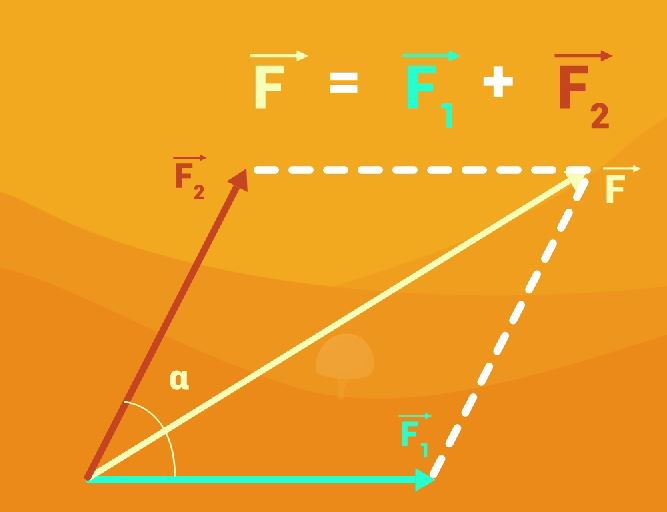
\includegraphics[scale=0.35]{../figs/VN10-PH-11-L-008-2-V2-01.jpg}
			\end{center}
	\end{itemize}

\manatip{
	Độ lớn hợp lực trong một số trường hợp đặc biệt:
\begin{itemize}
	\item Nếu $\vec{F}_1$ cùng chiều $\vec{F}_2$ $$F=F_1+F_2,$$
	\item Nếu $\vec{F}_1$ ngược chiều $\vec{F}_2$ $$F=|F_1-F_2|,$$
	\item Nếu $\vec{F}_1$ vuông góc $\vec{F}_2$ $$F=\sqrt{F_1^2+F_2^2}.$$
\end{itemize}
}


\subsection{Phân tích lực}
\begin{itemize}
	\item Phân tích lực là thay thế một lực bằng hai hay nhiều lực có tác dụng giống hệt như lực đó.
	\item Phân tích một lực thành hai lực thành phần đồng quy phải tuân theo quy tắc hình bình hành.
	%	\item Chỉ khi biết một lực có tác dụng cụ thể theo hai phương nào thì mới phân tích lực theo hai phương ấy. 
\end{itemize}
\subsection{Điều kiện cân bằng lực}
Muốn cho một chất điểm đứng cân bằng thì hợp lực của các lực tác dụng lên nó phải bằng không.
$$\vec{F}=\vec{F}_1+\vec{F}_2+...=\vec{0}.$$
\subsection{Mối liên hệ giữa lực và gia tốc}
Một vật chịu tác dụng của hợp lực khác không sẽ có gia tốc. Gia tốc này cùng chiều với lực, có độ lớn tỉ lệ thuận với độ lớn của lực và tỉ lệ nghịch với khối lượng của vật
\begin{equation*}
	\vec{a}=\dfrac{\vec F}{m},
\end{equation*}
trong đó:
\begin{itemize}
	\item $\vec F$ là lực tác dụng lên vật (N);
	\item m là khối lượng của vật (kg);
	\item $\vec a$ là gia tốc của vật ($\text{m/s}^2$).
\end{itemize}
\section{Mục tiêu bài học - Ví dụ minh họa}
\begin{dang}{Nhận biết đặc điểm của lực\\ và điều kiện hai lực cân bằng}
	\viduii{1}{Hai em học sinh A và B chơi kéo co. Sợi dây đứng yên. Chọn câu trả lời đúng:
		\begin{mcq}
			\item Lực mà hai đầu dây tác dụng lên hai tay của em học sinh là hai lực cân bằng.
			\item Lực mà hai học sinh tác dụng lên hai đầu của dây là hai lực cân bằng.
			\item Lực mà tay của học sinh A tác dụng lên đây và lực mà dây tác dụng lên tay A là hai lực cân bằng.
			\item A, B, C đều đúng.
		\end{mcq}
	}
	{	\begin{center}
			\textbf{Hướng dẫn giải}
		\end{center}
		Hai lực cân bằng phải cùng tác dụng lên một vật, nhưng không gây ra gia tốc cho vật ấy. 
		
		Đáp án A: hai lực này tác dụng lên hai vật khác nhau (là hai em học sinh) nên không phải hai lực cân bằng.\\ 
		Đáp án B: đây là hai lực cân bằng vì cùng tác dụng lên một vật (sợi dây) nhưng không gây ra gia tốc cho dây (dây đứng yên).\\ 
		Đáp án C: Hai lực không cân bằng vì không cùng tác dụng lên một vật: một lực tác dụng lên dây còn lực kia tác  dụng lên tay của em học sinh. \\
		Đáp án D: chỉ có B là đáp án đúng. 
		
		\textbf{Đáp án: B}.
	}
	\viduii{1}{Lựa chọn phương án đúng:
		
		Một học sinh đá vào một quả bóng cao su đang nằm yên trên mặt đất. Điều gì sẽ xảy ra sau đó:
		
		\begin{mcq}
			\item Quả bóng bị biến dạng.
			\item Quả bóng vẫn đứng yên.
			\item Quả bóng vừa biến dạng vừa biến đổi chuyển động.
			\item Quả bóng chỉ bị biến đổi chuyển động.
		\end{mcq}
	}
	{	\begin{center}
			\textbf{Hướng dẫn giải}
		\end{center}
		
		Quả bóng vừa biến dạng vừa biến đổi chuyển động.
		
		\textbf{Đáp án: C}.
	}
\end{dang}

\begin{dang}{Ghi nhớ đặc điểm hợp lực\\ của  hai lực đồng quy}
	\viduii{1}{Một chất điểm chịu tác dụng đồng thời của hai lực thành phần có độ lớn $F_1$ và $F_2$ thì hợp lực $\vec{F}$ của chúng luôn có độ lớn thỏa mãn hệ thức: 
		\begin{mcq}(2)
			\item $F = F_1^2 +F_2^2$.
			\item $|F_1 - F_2 |\leq F \leq F_1 +F_2.$
			\item $F = F_1+F_2.$
			\item $F = \sqrt {F_1^2+F_2^2}.$
		\end{mcq}
	}
	{	\begin{center}
			\textbf{Hướng dẫn giải}
		\end{center}
		
		Về độ lớn $|F_1-F_2|\leq F\leq F_1+F_2.$
		
		\textbf{Đáp án: B}.
	}
	\viduii{1}{Lực tổng hợp của hai lực đồng quy có giá trị lớn nhất khi 
		\begin{mcq}(2)
			\item Hai lực thành phần cùng phương, cùng chiều.      
			\item Hai lực thành phần cùng phương, ngược chiều.
			\item Hai lực thành phần vuông góc với nhau. 
			\item Hai lực thành phần hợp với nhau một góc khác không.
		\end{mcq}
	}
	{	\begin{center}
			\textbf{Hướng dẫn giải}
		\end{center}
		
	Hai vector cộng nhau tạo thành một vector có độ lớn cực đại khi hai vector đó cùng chiều với nhau. 
		
		
		\textbf{Đáp án: A}.
	}
\end{dang}

\begin{dang}{Tổng hợp lực \\theo quy tắc hình bình hành. }
	\viduii{2}{Tìm độ lớn hợp lực $\vec F$ của hai lực đồng quy $\vec{F}_1$ và $\vec{F}_2$ trong các trường hợp sau, nếu biết độ lớn $F_1=\SI{30}{N}$, $F_2=\SI{40}{N}$, góc giữa $\vec{F}_1$ và $\vec{F}_2$ là:
		\begin{enumerate}[label=\alph*.]
			\item $\alpha =0^\circ$.
			\item $\alpha =60^\circ$.
			\item $\alpha =90^\circ$.
			\item $\alpha =180^\circ$.
		\end{enumerate}
	}
	{	\begin{center}
			\textbf{Hướng dẫn giải}
		\end{center}
		
		\begin{enumerate}[label=\alph*.]
			\item Góc hợp bởi $\vec{F}_1$ và $\vec{F}_2$ là $\alpha =0^\circ$, tức là  $\vec{F}_1$ cùng chiều $\vec{F}_2.$
			
			Do đó, độ lớn $F=F_1+F_2= 70\, \si{\newton}$.
			\item Góc hợp bởi $\vec{F}_1$ và $\vec{F}_2$ là $\alpha =60^\circ.$
			
			Do đó, độ lớn $F=\sqrt{F_1^2+F_2^2+2F_1F_2\cos \alpha }= 10\sqrt{37}\,\si{\newton}$.
			\item Góc hợp bởi $\vec{F}_1$ và $\vec{F}_2$ là $\alpha =90^\circ$, tức là  $\vec{F}_1$ vuông góc $\vec{F}_2.$
			
			Do đó, độ lớn $F=\sqrt{F_1^2+F_2^2}=50\, \si{\newton}$.
			\item Góc hợp bởi $\vec{F}_1$ và $\vec{F}_2$ là $\alpha =180^\circ$, tức là  $\vec{F}_1$ ngược chiều $\vec{F}_2.$
			
			Do đó, độ lớn $F=|F_1-F_2|= 10\si{\newton}$.
		\end{enumerate}
		
	}
	\viduii{2}{Cho hai lực đồng quy có cùng độ lớn $\SI{9}{N}$. Góc giữa hai lực bằng bao nhiêu thì hợp lực cũng có độ lớn bằng $\SI{9}{N}$? 
	}
	{	\begin{center}
			\textbf{Hướng dẫn giải}
		\end{center}
		
		Độ lớn:
		$$F=\sqrt{F_1^2+F_2^2+2F_1F_2\cos \alpha }.$$
		$$\Rightarrow \cos \alpha = \dfrac{F^2-F_1^2-F_2^2}{2F_1F_2}= -\dfrac{1}{2}.$$
		$$\Rightarrow \alpha =120^\circ. $$
		
		Vậy góc giữa hai lực bằng $120^\circ.$
	}
\end{dang}
\begin{dang}{Ghi nhớ đặc điểm của phép phân tích lực}
	\viduii{1}{Khi nói về phép phân tích lực, phát biểu nào sau đây đúng?
		\begin{mcq}
			\item Phân tích lực là thay thế một lực bằng hai hay nhiều lực có tác dụng giống hệt như lực đó.
			\item Khi phân tích một lực thành hai lực thành phần thì phải tuân theo quy tắc tam diện thuận
			\item Khi phân tích một lực thành hai lực thành phần thì hai lực thành phần làm thành hai cạnh của tam giác.
			\item Phân tích lực là phép thay thế các lực tác dụng đồng thời vào vật bằng một lực như các lực đó.
		\end{mcq}
	}
	{	\begin{center}
			\textbf{Hướng dẫn giải}
		\end{center}
		
		Phân tích lực là thay thế một lực bằng hai hay nhiều lực có tác dụng giống hệt như lực đó.Các lực thay thế gọi là các lực thành phần. 
		
		A - đúng
		
		B – sai vì: Khi phân tích một lực thành hai lực thành phần thì phải tuân theo quy tắc hình bình hành
		
		C – sai vì chưa đầy đủ vị trí của hai cạnh này so với lực ban đầu.  
		
		D – sai, đây là phép tổng hợp lực. 
		
		\textbf{Đáp án: A}.
	}
	\viduii{1}{Điều nào sau đây là đúng khi nói về phép phân tích lực. 
		\begin{mcq}
			\item Phép phân tích lực là phép làm ngược lại với phép tổng hợp lực. 
			\item Phép phân tích lực tuân theo qui tắc hình bình hành.
			\item Phép phân tích lực là phép thay thế một lực bằng hai hay nhiều lực thành phần.   
			\item Cả A, B và C đều đúng.
		\end{mcq}
	}
	{	\begin{center}
			\textbf{Hướng dẫn giải}
		\end{center}
		
		Phân tích lực là thay thế một lực bằng hai hay nhiều lực có tác dụng giống hệt như lực đó. Các lực thay thế gọi là các lực thành phần. 
		
		\textbf{Đáp án: D}.
	}
\end{dang}

\begin{dang}{Phân tích lực\\ theo quy tắc hình bình hành}
	\viduii{2}{Một chất điểm chịu tác dụng đồng thời của hai lực thành phần vuông góc với nhau có độ lớn lần lượt là $F_1 = \SI{15}{N}$ và $F_2$. Nếu hợp lực có độ lớn là $\SI{25}{N}$ thì giá trị của $F_2$ là
		\begin{mcq}(4)
			\item $\SI{10}{N}$.
			\item $\SI{20}{N}$.
			\item $\SI{30}{N}$.
			\item $\SI{40}{N}$.
		\end{mcq}
	}
	{	\begin{center}
			\textbf{Hướng dẫn giải}
		\end{center}
		
		Nếu $\vec{F}_1$ vuông góc $\vec{F}_2$ thì hợp lực sẽ có độ lớn 
				$$F=\sqrt{F_1^2+F_2^2} \quad\Rightarrow\quad F_2=\sqrt{F^2-F_1^2}.$$
		
		Thay các giá trị số từ đề bài, độ lớn hợp lực có giá trị 		
		$$F_2 = \sqrt {F^2 - F_1^2} =\sqrt{(\SI{25}{\newton})^2-(\SI{15}{\newton})^2}= \SI{20}{N}.$$
		
		\textbf{Đáp án: B}.
	}
	\viduii{2}{Cho lực $F$ có độ lớn $\SI{100}{N}$ và có hướng tạo với trục Ox một góc $\SI{36,87}{^\circ}$ và tạo với Oy một góc $\SI{53,13}{^\circ}$. Xác định độ lớn các thành phần của lực $F$ trên các trục Ox và Oy.
	}
	{	\begin{center}
			\textbf{Hướng dẫn giải}
		\end{center}
		
%		Độ lớn của góc hợp bởi Ox và Oy
		
%		$$\SI{36,87}{^\circ} + \SI{53,13}{^\circ}= \SI{90}{^\circ}$$
		
		Độ lớn các thành phần của lực $F$
		\begin{align*}
			F_{x} &= F\cos \SI{36,87}{^\circ} = \SI{80}{N}\\
			F_{y}&= F\cos \SI{53,13}{^\circ} = \SI{60}{N}
		\end{align*}
	}
\end{dang}
\begin{dang}{Tính các lực tác dụng lên vật \\khi vật cân bằng}
	\viduii{3}{Một vật có trọng lượng $P= 10$ N. được treo vào một vòng nhẫn O (coi là chất điểm). Vòng nhẫn được giữ yên bằng hai dây OA và OB. Biết dây OA nằm ngang và hợp với dây OB một góc $120^\circ.$ Tìm lực căng dây của hai dây OA và OB.
		
		\begin{center}
			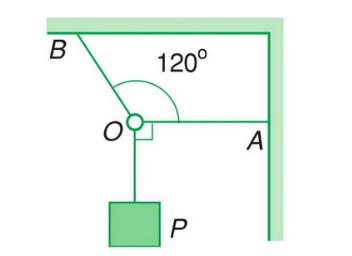
\includegraphics[scale=0.5]{../figs/VN10-PH-11-L-008-4-V2-01.jpg}
		\end{center}
	}
	{	\begin{center}
			\textbf{Hướng dẫn giải}
		\end{center}
		
		\begin{center}
			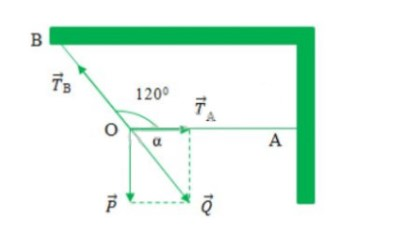
\includegraphics[scale=0.8]{../figs/VN10-PH-11-L-008-4-V2-02.jpg}
		\end{center}
		Khi vật ở vị trí cân bằng thì các lực tác dụng lên vật gồm trọng lực $\vec{P}$, lực căng trên hai dây $\vec{T}_A$ và $\vec{T}_B$. Vòng nhẫn đứng yên nên các lực cân bằng nhau
		$$\vec{P}+\vec{T}_\textrm{A}+\vec{T}_\textrm{B}=\vec{0}.$$
		Gọi $\vec{Q}$ là hợp lực của $\vec{P}$ và $\vec{T}_A$
		$$\vec{P}+\vec{T}_\textrm{A}=\vec{Q}\quad\Rightarrow \quad\vec{T}_\textrm{B}+\vec{Q}=\vec{0}\quad\Rightarrow\quad \vec{T}_\textrm{B}=-\vec{Q}$$
		nghĩa là $\vec{Q}$ và $\vec{T}_B$ là hai vector trực đối. Do đó, $\alpha =\SI{	180}{\degree}-\SI{120}{\degree}=\SI{60}{\degree}.$
		
		Xét $\triangle$O$T_\text{A}$Q vuông tại $T_\text{A}$:
		
		$$\tan \alpha =\dfrac{P}{T_\text{A}}\Rightarrow T_\text{A}=\dfrac{P}{\tan \alpha}=\dfrac{10\sqrt{3}}{3}\,\text{N}.$$
		$$\sin \alpha =\dfrac{P}{Q}\Rightarrow Q=\dfrac{P}{\sin \alpha}=\dfrac{20\sqrt{3}}{3}\,\text{N}.$$
		Vì $|\vec{T}_\textrm{B}|=|\vec{Q}|$ nên $T_\textrm{B}= \dfrac{20\sqrt{3}}{3}\,\text{N}.$
		
		Vậy lực căng dây của hai dây OA và OB lần lượt bằng $\dfrac{10\sqrt{3}}{3}\,\text{N}, \dfrac{20\sqrt{3}}{3}\,\text{N}.$
	}
	\viduii{3}{Một đèn tín hiệu giao thông ở đại lộ có trọng 
		lượng 120 N được treo vào trung điểm của dây 
		AB làm dây thòng xuống $\text{0,5}$ m. Cho biết hai trụ treo dây cách nhau \SI{8}{\meter}, bỏ qua 
		trọng lượng của dây, tính lực căng mỗi sợi dây. 
		\begin{center}
			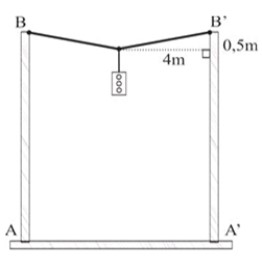
\includegraphics[scale=0.7]{../figs/VN10-PH-11-L-008-4-V2-03.jpg}
		\end{center}
	}
	{	\begin{center}
			\textbf{Hướng dẫn giải}
		\end{center}
		
		\begin{center}
			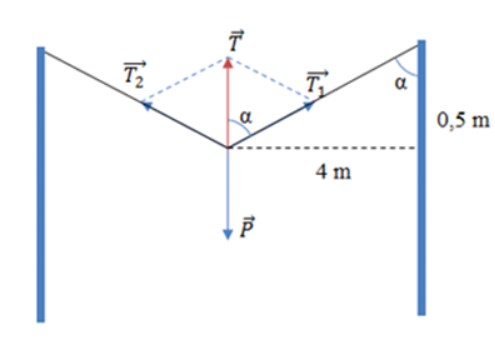
\includegraphics[scale=0.5]{../figs/VN10-PH-11-L-008-4-V2-04.jpg}
		\end{center}
		Đèn khi cân bằng chịu các lực tác dụng như hình vẽ, gồm trọng lực $\vec{P}$, hai lực căng dây $\vec{T}_1$ và $\vec{T}_2$
			\begin{align*}
				\vec{P}+\vec{T}_1+\vec{T}_2=0
			\end{align*}
		
		Gọi $\vec T$ là hợp lực của hai dây cáp:
		$$\vec{T}=\vec{T}_1+\vec{T}_2\quad\Rightarrow\quad \vec{P}+\vec{T}=0$$
		nghĩa là $T=P=mg=\SI{120}{\newton}$.
		
		Do tính đối xứng, hai lực căng dây phải có độ lớn bằng nhau $T_1=T_2$. Từ hình vẽ 
			\begin{align*}
				T=2T_1\cos \alpha\quad\Rightarrow\quad T_1=\dfrac{T}{2\cos\alpha}
			\end{align*}
		trong đó góc $\alpha$ được xác định từ tam giác vuông bên phải trên hình
			\begin{align*}
				\tan\alpha=\dfrac{\SI{4}{\meter}}{\SI{0.5}{\meter}}=8\quad\Rightarrow\quad \alpha\approx\SI{82.875}{\degree}. 
			\end{align*}
		Từ đó ta tính được lực căng dây
			\begin{align*}
				T_1=T_2=\dfrac{T}{2\cos\alpha}\approx \SI{484}{\newton}.
			\end{align*}		
% Hung comment: bài giải cũ sai bước thế số: sử dụng giá trị trọng lực là 60N 
	}
	
	
\end{dang}
\begin{dang}{Áp dụng mối liên hệ giữa lực và gia tốc của vật chuyển động thẳng biến đổi đều}
	\viduii{2}{Một ô tô có khối lượng 3 tấn, sau khi khởi hành 10 giây thì đi được quãng đường 25 m. Bỏ qua ma sát, tìm:
		\begin{enumerate}[label=\alph*.]
			\item Lực phát động của động cơ xe.  	
			\item Vận tốc và quãng đường xe đi được trong 20 s.  
		\end{enumerate}
	}
	{	\begin{center}
			\textbf{Hướng dẫn giải}
		\end{center}
		
		\begin{enumerate}[label=\alph*.]
			\item Gia tốc của xe được xác định từ phương trình chuyển động 
				$$s=\dfrac{1}{2}at^{2}\quad\Rightarrow\quad a=\dfrac{2s}{t^2}=\dfrac{2\cdot\SI{25}{\meter}}{(\SI{10}{\second})^{2}}=\SI{0.5}{\meter/\second^{2}}.$$
			Lực phát động của xe có độ lớn 
				\begin{align*}
					F=ma=\SI{3000}{\kilogram}\cdot\SI{0.5}{\meter/\second^2}=\SI{1500}{\newton}.
				\end{align*}
			\item Vận tốc của xe sau 20 giây 			$$v=v_0+at=\SI{0}{\meter/\second}+(\SI{0.5}{\meter/\second^2})\cdot(\SI{20}{\second})=\SI{10}{\meter/\second}.$$
			Quãng đường xe đi được trong thời gian tương ứng
			$$s=\dfrac{1}{2}at^2=\dfrac{1}{2}\cdot(\SI{0.5}{\meter/\second^2})\cdot(\SI{20}{\second})^2=\SI{100}{\meter}.$$  
		\end{enumerate}	
		
	}
	\viduii{2}{Một vật có khối lượng 2 kg đang chuyển động với tốc độ 1 m/s thì chịu tác dụng bởi một lực cùng hướng chuyển động và có độ lớn $F$. Biết rằng sau đi được 1 m, vật đạt tốc độ 2 m/s. Tìm độ lớn lực $F$.
		
	}
	{	\begin{center}
			\textbf{Hướng dẫn giải}
		\end{center}
		Áp dụng công thức liên hệ giữa quãng đường, vận tốc, gia tốc với các giá trị $s= \SI{1}{\meter}$, $v= \SI{2}{\meter/\second}$, $v_0=\SI{1}{\meter/\second}$, ta tìm được gia tốc của vật 
			\begin{align*}
				v^2-v_0^2=2as \quad\Rightarrow\quad a=\dfrac{v^2-v_0^2}{2s}=\dfrac{(\SI{2}{\meter/\second})^2-(\SI{1}{\meter/\second})^2}{2\cdot\SI{1}{\meter}}=\SI{1.5}{\meter/\second^2}.
			\end{align*}
		Lực tác động có độ lớn 
			\begin{align*}
				F=ma=\SI{2}{\kilogram}\cdot\SI{1.5}{\meter/\second^2}=\SI{3}{\newton}.
			\end{align*}		
	}
\end{dang}